\documentclass[12pt,a4paper,titlepage]{article}
\usepackage[utf8]{inputenc}
%\usepackage[finnish]{babel}
\usepackage{setspace}
\usepackage{parskip}
\usepackage{amssymb}
\usepackage{amsmath}
\usepackage{graphicx}
\usepackage{fancyhdr}
\usepackage[top=1in, bottom=1in, left=1in, right=1in]{geometry}
\usepackage{float}
\usepackage[section]{placeins}
\usepackage{listings}
\usepackage{courier}
\usepackage{subcaption}
\usepackage{textcomp}
%\usepackage[numbered,autolinebreaks,useliterate]{mcode} % jos tahdot laittaa matlabkoodia näkyville niin kannattaa käyttää tätä

% hyödyllisiä paketteja:
%\usepackage{siunitx}\sisetup{per=frac} % SI-yksiköitä.
%\usepackage{supertabular} % jos tarttee isoja taulukoita
%\usepackage{fullpage} % pienemmät marginaalit jos haluaa

\lstset{basicstyle=\ttfamily,breaklines=true,xleftmargin=.25in}

\usepackage{hyperref} % lisääthän omat pakettisi ENNEN hyperref'iä
\hypersetup{pdfborder={0 0 0}}
\onehalfspacing
\cfoot{}
\rhead{\thepage}
% asettaa nyk. kappaleen nimen vasempaan ylänurkkaan, saa poistaa jos haluaa
\lhead{\leftmark}

%%%%% kaikki ennen tätä liittyy käytettäviin paketteihin tai dokumentin muotoiluun. siihen ei tarvinne aluksi koskea. %%%%%

%%%%% kansilehti %%%%%
\title{Scientific Computing III \\ Restricted three-body problem \vspace{0.5em}}
\author{Anni Järvenpää}
\date{\today}
\begin{document}
\maketitle

% Sisällysluettelo
\newpage
\thispagestyle{empty}
\tableofcontents
\newpage
\setcounter{page}{1}
\parskip=1em \advance\parskip by 0pt plus 2pt
\pagestyle{fancy}

% prosenttimerkillä alkavat rivit ovat kommentteja: niitä ei katsota dokumenttia käännettäessä eli ne ovat vain kirjoittajaa varten

%%%%%%%%%%%%%%% Oleellinen sisältö alkaa%%%%%%%%%%%%%%%

\section{Introduction}
% Describe the problem and its background and motivation.
The restricted three-body problem is a problem conserning the movement of an object of negligible mass near two massive objects. Due to the small mass of the third body (denoted $m_3$ from now on), the primaries $m_1$ and $m_2$ can be considered to be on Keplerian orbits. Therefore the two primaries can be on circular, elliptical, parabolic or hyperbolic orbits relative to each other, which affects the possible orbits for $m_3$. \cite{dj}

Especially the circular case is interesting, because it is simple enough to be fairly well understood and it can be used as an approximation for the interactions of Sun, a planet and a small body such as meteoroid or a comet. Especially Jupiter dominates the orbits of many small bodies in our Solar System. As we will later find out, some points in this three-body system are stable, which is a property that can be used to keep spacecraft stable relative to Earth-Sun pair. For example GAIA is on an orbit that keeps it behind Earth as viewed from the Sun and SOHO orbits the Sun staying always between Earth and Sun and thus getting unobstructed view of the Sun. \cite{dj, gaia, soho}

\section{Theoretical Background}\label{theory}
Due to the complexity of general case, we will only analyze the planar circular restricted three-body problem. This means that the primaries are on circular orbits and the orbit of the third mass lies in the same plane as the orbit of the primaries.

The burden of cumbersome calculation work can be greatly relived by choosing units and coordinate system carefully. In this case, a good choice is a cartesian ($x$, $y$) coordinate system that rotates with the primaries such that the primaries always lie on the x-axis. This can be achieved by positioning the mass centre of the primaries to the origin. Choosing the direction of positive $x$-axis is arbitrary, but let's fix the more massive primary to reside on the negative axis. Now the coordinate system ($x$, $y$) rotates at an angular velocity $n$ relative to the inertial ($x_{inertial}$, $y_{inertial}$) coordinate system. Coordinate system like this is shown in figure \ref{coordinates}.

\begin{figure}
\centering
\includegraphics[width=0.8\textwidth]{../plots/coordinates.png}
\caption{Rotating coordinate system.}
\label{coordinates}
\end{figure}

The situation can be further simplified by choosing units wisely. Let's take the unit of mass to be the combined mass of the primaries, i.e. $m_1+m_2 = 1$. Now we can denote the mass of the smaller primary by $\mu$ and the larger by $1-\mu$. Due to the centre of mass being at the origin, the coordinates of the primaries are now fixed to $(1-\mu, 0)$ and $(-\mu, 0)$. Earlier we defined the angular velocity at which the coordinate system rotates to be $n$, so it is natural to choose the unit of time to be the orbital period of the primaries divided by $2\pi$ since then $n=1$. Now that the total mass of the system, $n$ and semimajor axis of the orbit are 1, gravitational constant $G$ must also be 1. These conventions make the calculations simple and this unit system will be used in simulations too.

In an inertial coordinate frame a third body placed near the primaries would simply obey Newton's second law. In rotating coordinate frame one must also consider ''fictious'' Coriolis and centrifugal forces. Due to them the acceleration in inertial frame $\vec a_{i}$ in Newton's second law
\begin{equation}
	\vec F_i = m\vec a_i
\end{equation}
has to be replaced with
\begin{equation}\label{accelerations}
	\vec a_i = \vec a_r + 2\vec n \times \vec v_{r} + \vec n \times ( \vec n \times \vec r)
\end{equation}
where $\vec n$ is the angular velocity vector of the rotating frame and $\vec a_r$ and $\vec v_r$ are acceleration and velocity relative to the rotating frame. In equation \ref{accelerations} the second term corresponds to the Coriolis force and the third to the centrifugal force. \cite{dj}

From this and clever use of knowledge about mechanics in rotating frame we get expression for gravitational potential in rotating coordinate frame:
\begin{equation}
	V = -\frac{1-\mu}{r_1} - \frac{\mu}{r_2}
\end{equation}
where $r_1$ and $r_2$ are lengths of vectors $\vec r_1$ and $\vec r_2$ from figure \ref{coordinates}. Coriolis effect affects only moving particles and thus it does not affect the value of potential but centrifugal force adds a term $r/2$ and thus we get an expression for effective potential in rotating frame:
\begin{equation}
	U = -\frac{1}{2}r - \frac{1-\mu}{r_1} - \frac{\mu}{r_2}.
\end{equation}
This can be used to calculate the force a stationary body in rotating coordinate frame feels but when a particle gains velocity the Coriolis effect will cause it to feel force that deviates from $-\nabla U$ as we will see from the simulation results presented later. \cite{dj}

Shape of the effective potential around the primaries is shown in figure \ref{potential}. Near the primaries the gravitational potential of the closest body dominates but further away the centrifugal effect gets more important. Already from this plot we can find five points, where a stationary body will remain stationary. None of these are stable, because all of them are either saddle points or potential maxima, but as we will later see the Coriolis effect can stabilize some orbits near these points. \cite{dj}

Three of these stationary points lie on the line connecting the primaries, one on either side of them and one in between, and the last two form equilateral triangles with the primaries. These points are known as Lagrangian points and it is customary to number them from 1 to 5. Conventions vary somewhat, but a common numbering scheme is to number them from the smallest potential to the largest, thus having L1 between the primaries, L2 on the far side of the smaller primary, L3 on the far side of the larger primary and L4 and L5 at triangular points. \cite{dj}

\begin{figure}
\centering
\includegraphics[width=0.7\textwidth]{../plots/potential.png}
\caption{Effective potential around the two primaries.}
\label{potential}
\end{figure}

We have an expression for the effective potential for an object, but the actual orbit of the third particle has no closed-form expression in general case. Nevertheless, we can express some restrictions for the orbit of the third body based on its energy. We know it's kinetic energy to be $v^2/2$ and therefore from the law of conservation of energy we know that
\begin{equation}
	\frac{1}{2}v^2 + U = C
\end{equation}
where $C$ is a constant known as Jacobi constant or Jacobi integral. Often this is shown with both sides of the equation multiplied by 2. Then we get a new constant $2C$ that some sources call Jacobi constant. \cite{dj, tm}

If we know the position and velocity of an object at some time, we can easily calculate the value of $C$. In three-body situation the value of $C$ will remain constant for the lifetime of the body and therefore it implies limits for the area where the third body can be found. For all physical cases, $v \geq 1$ so the body can only move in parts of the space where \cite{dj, tm}
\begin{equation}
	U \leq \frac{C}{2}.
\end{equation}



Figures \ref{open}--\ref{closed} show areas a test particle can reach for different values of C in a system where primaries resemble Sun and Jupiter ($\mu = 1/1047$). Top row plots in figure \ref{open} show forbidden areas forming first around L4 and L5 and then stretching longer as the energy of the orbit decreases. On the next row these vaguely tadpole-shaped forbidden areas connect at L3 and then grow together forming a horseshoe-shaped area.

\begin{figure}
\centering
\includegraphics[width=\textwidth]{../plots/allowed/open.png}
\caption{Tadpole and horseshoe shaped forbidden areas.}
\label{open}
\end{figure}

In figure \ref{zooms} we can see how the horseshoe closes in to form a circle, first connecting at L2 and dividing the space where the third mass can move to two distinct parts (top row). Then on the second row we see the forbidden area closing up on L1 and leaving the particle three areas where it can move: around the more massive primary, around the less massive primary or on a large orbit around both of them. It is clear that the third mass cannot move from one of these areas to another, because it would have to travel through an area where it would have negative velocity. When the energy of the orbit decreases further the forbidden areas grow as can be seen in figure \ref{closed}.

\begin{figure}
\centering
\includegraphics[width=\textwidth]{../plots/allowed/zooms.png}
\caption{Forbidden areas closing first on L2 and then on L3.}
\label{zooms}
\end{figure}


\begin{figure}
\centering
\includegraphics[width=\textwidth]{../plots/allowed/closed.png}
\caption{Forbidden areas divide space to three distinct areas: Solar orbit, Jovian orbit or a large orbit around both of them.}
\label{closed}
\end{figure}

Naturally this analysis offers us no information about which parts of space the test mass will actually reach. Even though a mass with small initial velocity at L4 has enough energy to travel anywhere in the system, it might be on an orbit that will instantly escape the system or it might be on an orbit that will keep it close to the primaries or close to the L4 point for long times. This is where numerical simulations are needed.


\section{Methods}
%  Describe (if applicable) the model, theoretical methods, and numerical methods that you use. 
Leapfrog integrator is a numerical integrator that is well suited for dynamical systems and classical mechanics. The name comes from velocities and positions of particles being updated alternately with half a timestep between successive updates. It is possible to implement in kick-drift-kick or drift-kick-drift form, former of which is described belos. Accelerations of the particles are first calculated for the current positions of particles. Then the velocities are calculated after half a timestep has passed, i.e.
\begin{equation}
	v_{t+\Delta t/2} = v_t + a_t\frac{\Delta t}{2}.
\end{equation}
This new value of $v$ is then used to calculate the positions of the bodies after one timestep has elapsed:
\begin{equation}
	x_{t+\Delta t} = x_t + v_{t+\Delta t/2}\Delta t
\end{equation}
Last the accelerations in the new position are calculated and velocity is updated for the other half of the timestep:
\begin{equation}
	v_{t+\Delta t} = v_{t+\Delta t/2} + a_{t+\Delta t}\frac{\Delta t}{2}.
\end{equation}
If output is not desired after every timestep, it is possible to calculate the kick-steps at one step of length $\Delta t$ and synchronizing the velocities and positions only when an output is desired. \cite{dj, wikifrog}

For numerical equation solving I used Matlab function vpasolve.


\section{Implementation of the methods}
% Describe the program written for the project 
% and/or the existing software (programs, libraries) used. Give instructions on 
% how to compile and use the program so that the reader is able to reproduce 
% your results. Do not attach the program source code to the report. 

For finding the Lagrangian points and plotting their locations I created a Matlab script \texttt{lagrangesolver.m} that can be found under \texttt{plottaus} directory or via direct link \url{https://github.com/aajarven/tilaIII/blob/master/lopputyo/plottaus/lagrangesolver.m}. It goes through different values of $\mu$ between 0 and 1 finding solutions for equations
\begin{align*}
x - \frac{1-\mu}{(x+\mu)^2} - \frac{\mu}{[x-(1-\mu)]^2} &= 0 \\
x - \frac{1-\mu}{(x+\mu)^2} + \frac{\mu}{[x-(1-\mu)]^2} &= 0 \\
x + \frac{1-\mu}{(x+\mu)^2} + \frac{\mu}{[x-(1-\mu)]^2} &= 0 
\end{align*}
in ranges $1-\mu<x$, $-\mu<x<1-\mu$ and $x<-\mu$ respectively. Locations are saved in vectors \texttt{x1}, \texttt{x2} and \texttt{x3} from where they can easily be plotted together with the values of $\mu$ they correspond to.

For studying the motion of a satellite near the Lagrangian points I implemented a leapfrog integrator with C using an integrator I made for Advanced Dynamics course as a starting point (original available online at \url{https://github.com/aajarven/ad-integrators}). It uses the leapfrog integrator described above with synchronizing done after every timestep. I removed unnecessary parts, changed the code to work on 2D case, removed unit conversions to allow use of the units described in section \ref{theory} and created new input files in addition to some small changes. Resulting program can be found and downloaded from \url{https://github.com/aajarven/tilaIII/tree/master/lopputyo}.

Source files together with a makefile can be found in src directory. Program has been tested using GNU compiler and C99 standard. Just typing \texttt{make} in \texttt{src} directory should compile the program and place the executable in (pre-existing!) \texttt{bin} directory under \texttt{lopputyo}. Some input files can be found in \texttt{input} directory, for example \texttt{input/input\_atL2.dat} has initial conditions for situation where test mass is located at the L2 point. It is also simple to create custom input files: the program expects the input files to contain one line per object with each line having x and y positions, x and y velocities and mass in this order separated by spaces. The integration is carried out in inertial coordinate frame, but if one wishes to use my plotting scripts it is important that the primaries are on first rows, because otherwise when plotting is done in rotating coordinate frame, the frame might rotate with the test particle and thus create wonky orbits.

After compiling the program can be run using commands of the form
\begin{lstlisting}
./bin/main input/input_atL2.dat 3 0.0001 1 2 run/out.dat
\end{lstlisting}
which uses input file \texttt{input/input\_atL2.dat} that contains three bodies, runs the simulation for 1 time unit (Jovian year in this case) using 0.0001 time unit timesteps and outputs the state of the simulation to file \texttt{run/out.dat} on every other time step. Trying to run the program with fewer arguments causes it to show a message with short instructions. Using too many or incorrect arguments may cause an unhandled crash and is not recommended.

The output files contain state of one body at one time per line, each line being of the form
\begin{lstlisting}
bodyIndex;	time;	x,	y;	vx,	vy;
\end{lstlisting}
i.e. every piece of data is separated with a tab and either a semicolon or a comma. Numbers on the first column run from 0 to number of bodies in simulation - 1, each simulation body having a unique index.

\section{Results}
% If applicable comment on the accuracy of the results and on the efficiency of the method/program. 
\subsection{Location of the Lagrangian points}
Locations of the L4 and L5 points are readily available with simple trigonometry: in the rotating coordinate system described in section \ref{theory} their x-coordinate will be the mean of the primaries x-coordinates and the y-coordinates will be $\pm0.5 \tan{60^{\circ}}$. Locations of the three other Lagrangian points as a function of the mass ratio of the primaries are more complex. Therefore I used a numerical solver to solve their locations at different $\mu$'s, result of which is can be seen in figure \ref{Lpoints}. The ''Sun'' is shown to be always on the negative x-axis though naturally as $\mu$ grows the ''planet'' will gradually be more massive. Therefore at $\mu = 0.5$ the definitions of Sun and planet (and L3 and L2) will change places. Nevertheless the plot is shown up to $\mu = $ because it makes it easier to see the symmetry of the situation.

\begin{figure}
\centering
\includegraphics[width=\textwidth]{../plots/Lpoints.png}
\caption{Locations of the first three Lagrangian points relative to the primaries as a function of the mass ratio of the primaries.}
\label{Lpoints}
\end{figure} 

In the figure we can see how the L3 moves closer to the more massive body as its mass decreases, reaching their halfway point when the primaries have equal masses, This can be easily understood if it is considered as the point where the gravities of the two primaries exactly balance each other out. L2 and L3 have locations that stay more stable, not deviating very far from values 1 and -1.

\subsection{Movement of a test mass around the Lagrangian points of Sun-Jupiter system}\label{lagrangemovements}
To study the behaviour of a massless test particle at or near different Lagrangian points, I started by creating initial conditions corresponding to the primaries with $\mu=1/1047$ on x-axis and a test mass at different Lagrangian points with velocity corresponding to the rotation of the rotating coordinate frame. Then I did some runs with slightly perturbed velocities and/or positions to study what a small change in initial condition does to the orbit. All results are presented in the rotating coordinate system. Initial conditions producing plots presented below can be found in \texttt{inputs} directory and after reading the x and y vectors from the output file to Matlab the plots can be produced using orbitPlotter function located at the \texttt{plottaus} directory.

\subsubsection{L1}
For the L1 point I did not manage to find initial conditions that would have resulted in the test mass staying neatly at L1. The position and velocity I calculated for the test mass in L1 resulted in an orbit seen in figure \ref{L1-stable}. The shape of the orbit suggests that due to a small error the test mass was not precisely at the L1 and did not have enough energy to climb over the potential wall near L1, therefore corresponding to second row in figure \ref{zooms} where the test mass is confined to orbit the Sun at an orbit inside that of Jupiter.

The pointy ends at the outer parts of the orbit correspond to the particle getting close to the forbidden area. There its comes close to a halt in the rotating coordinate frame and starts falling back closer to the sun while the Coriolis effect slightly bends its orbit. In inertial coordinate system these would correspond to the apoapsides of the almost elliptical orbits.

Another possible distinct orbit is presented in figure \ref{L1-right}, where the test mass was placed slightly closer to Jupiter than the L1. It was not given the extra velocity to climb over the potential wall at L1, so now it is confined to the small region surrounding Jupiter in lower right plot of figure \ref{zooms}. A third case where the test mass is given a bit more velocity at L1 is shown at figure \ref{L1-morevel}. There it has enough energy to move from an orbit around Jupiter to another around Sun and it does so within the 50 Jovian year simulation period.

The amount of extra speed is not big enough to allow it to cross L2 or L3 and therefore it is confined to the region shown in upper row of \ref{zooms}. If the simulation was continued long enough, it would possibly have crossed the L1 and returned to an orbit around Jupiter or had the initial conditions been slightly different it could have orbited the Sun in the beginning and then moved to an orbit around Jupiter.

\begin{figure}
\centering
\includegraphics[width=0.7\textwidth]{../plots/L1-stationary.png}
\caption{Orbit of the test mass resulting from placing it approximately to L1.}
\label{L1-stable}
\end{figure}

\begin{figure}
\centering
\includegraphics[width=0.7\textwidth]{../plots/L1-right.png}
\caption{Orbit of the test mass resulting from placing it close to L1 but slightly closer to Jupiter.}
\label{L1-right}
\end{figure}

\begin{figure}
\centering
\includegraphics[width=0.7\textwidth]{../plots/L1-morevel.png}
\caption{Orbit of the test mass resulting from placing it to L1 but giving it a small amount of extra velocity.}
\label{L1-morevel}
\end{figure}

\subsection{L2}
For L2 my calculations gave a location that was precise enough to keep the test mass very close to L2 for the whole 1000 year simulation period as can be seen in figure \ref{L2-stationary}. More interesting orbits can be seen in figures \ref{L2-left} and \ref{L2-morevel}. In the first one the test mass is slightly closer to Jupiter than L2 and it starts at rest relative to the primaries. This means that it does not quite have the energy to cross L2 and hence the orbit resembles the one in figure \ref{L1-morevel}.

In the latter the test mass is initially at L2 but it has a small velocity relative to the primaries. This means that it is energetically possible for it to be anywhere in the white area of lower right plot of figure \ref{open}. When the excess energy at L2 is small, the hole in the forbidden area surrounding L2 is very small, which means that transitioning from outside the horseshoe-shaped forbidden area to the inside is very difficult. This is why I was not able to reconstruct an orbit that would reach the inner orbits in reasonably short time even though they would be theoretically possible and the test mass in the plot always stays outside orbit of Jupiter.

In this figure the pointy ends of the orbit at the inner perimeter correspond to the test mass getting close to the forbidden area from outside, its velocity decreasing and it starting to fall down the potential hill outwards from the primaries while as its velocity increases the Coriolis effect rotates its direction. In inertial coordinate frames these pointy ends would correspond to periapsides of the nearly-ellipsoidal orbit.

\begin{figure}
\centering
\includegraphics[width=0.7\textwidth]{../plots/L2-stationary.png}
\caption{Test mass (small black dot to the right of Jupiter) staying neatly at L2.}
\label{L2-stationary}
\end{figure}

\begin{figure}
\centering
\includegraphics[width=0.7\textwidth]{../plots/L2-orbitsboth.png}
\caption{Test mass initially at rest a bit closer to Jupiter than L2}
\label{L2-left}
\end{figure}

\begin{figure}
\centering
\includegraphics[width=0.7\textwidth]{../plots/L2-right.png}
\caption{One possible orbit for test mass that has a small initial velocity at L2}
\label{L2-morevel}
\end{figure}

\subsection{L3}
For L3 I could not find a perfectly stable orbit either, closest orbit is shown in figure \ref{L3-stable}. The slight deviation from ideal initial conditions causes the test mass to travel close to the zero-velocity curve surrounding the forbidden area in lower left plot in figure \ref{open}. When the test mass is moved a bit further than L3 its orbit will become bigger as can be seen in figure \ref{L3-left} and it can no longer penetrate the potential wall at L3. Moving it closer to the Sun would have resulted in an orbit resembling one seen in figure \ref{L2-left} where it cannot penetrate L3 but is inside the horseshoe-shaped forbidden area.

Due to energy in L3 being higher than in L2 or L1 choosing initial position and velocity near L3 carefully (or with sheer luck) will allow the test mass to move through the hole near L2 and L1 and transit to orbit inside the horseshoe as can be seen in figure \ref{L3-left2}. Now that the energy of the orbit is larger the allowed orbits around Jupiter are bigger. If the orbit has the necessary energy to move over the L3 point, a similar transition is possible through it too.

\begin{figure}
\centering
\includegraphics[width=0.7\textwidth]{../plots/L3-stationary.png}
\caption{Test mass initially as close to L3 as I could get.}
\label{L3-stable}
\end{figure}

\begin{figure}
\centering
\includegraphics[width=0.7\textwidth]{../plots/L3-left.png}
\caption{Orbit of a test mass initially a bit further away than L3.}
\label{L3-left}
\end{figure}

\begin{figure}
\centering
\includegraphics[width=0.7\textwidth]{../plots/L3-left3-100yr.png}
\caption{Orbit starting near L3 transitioning to inside the horseshoe-shaped forbidden area.}
\label{L3-left2}
\end{figure}

\subsection{L4 and L5}
Orbits near L4 and L4 closely resemble each other and therefore they will be considered together. Near those points I was able to produce a reasonably stable orbit where the test mass stays very close to its Lagrangian point as can be seen from figures \ref{L4-stationary} and \ref{L5-stationary} where motions of the test mass are shown over a period of 1000 Jovian years. The closer views of these orbits (shown in figures \ref{L4-zoom} and \ref{L5-zoom}) show the movements of the test mass.

In both cases the test mass makes nearly elliptical orbits around the rim of the potential well with Coriolis force causing the orbit to turn and stay close to the rim. As we can see, there is no forbidden region inside the orbit, which means that the particle would have enough energy to leave the system. This clearly illustrates that even if a particle has enough energy to be somewhere and there are no potential barriers preventing the movement, it won't necessarily ever end up there.

\begin{figure}
\centering
\includegraphics[width=0.7\textwidth]{../plots/L4-stationary.png}
\caption{Test mass staying near L4.}
\label{L4-stationary}
\end{figure}

\begin{figure}
\centering
\includegraphics[width=0.7\textwidth]{../plots/L5-stationary.png}
\caption{Test mass staying near L5.}
\label{L5-stationary}
\end{figure}

\begin{figure}
\centering
\includegraphics[width=0.7\textwidth]{../plots/L4-stationary-zoom.png}
\caption{Closer view on the test orbit of test mass near L4.}
\label{L4-zoom}
\end{figure}

\begin{figure}
\centering
\includegraphics[width=0.7\textwidth]{../plots/L5-stationary-zoom.png}
\caption{Closer view on the test orbit of test mass near L5.}
\label{L5-zoom}
\end{figure}

Due to the symmetry of L4 and L5, the following review is done only on particles near L4. In figures \ref{L4-tadpole} and \ref{L4-largertadpole} we see two somewhat tadpole-shaped orbits following the rim of the potential well of the planets. They are a natural extension to the very small but similarly shaped orbits seen previously and the same effect keeps the particles in their confined orbits. It is interesting to see how a particle can move on a fairly large area but still not go all the way around the system.

\begin{figure}
\centering
\includegraphics[width=0.7\textwidth]{../plots/L4-closerToOrigin.png}
\caption{Small tadpole-shaped orbit near L4.}
\label{L4-tadpole}
\end{figure}

\begin{figure}
\centering
\includegraphics[width=0.7\textwidth]{../plots/L4-evenCloserToOrigin.png}
\caption{Larger orbit around L4.}
\label{L4-largertadpole}
\end{figure}

If the tadpole-shaped orbit gets large enough, the ones corresponding to L4 and L5 will merge and result in a horseshoe-shaped orbit similar to one that can be seen in figure \ref{L4-horsie2}. If a particle starts from L4, it has enough energy to transit from one side of the horseshoe to another from the hole at L3, but for small excess energies the hole is again small and the transit is improbable which again separates horseshoe orbits from tadpole shaped ones. For somewhat horseshoe shaped orbits it is also possible for the test mass to jump over L2 hole as can be seen in figure \ref{L4-horsie1}.

It is also easily noticeable how in the rotating coordinate frame the orbits inside the horseshoe go counter-clockwise and orbits outside the horseshoe turn clockwise. This of course is not related to any actual major change of direction in the orbit of the test mass when it comes close to Jupiter but due to the fact that outside the orbit of Jupiter the test mass moves slower than the rotating coordinate system rotates relative to the inertial one whereas inside the orbit of Jupiter the test mass moves faster than the coordinate axes rotate.

\begin{figure}
\centering
\includegraphics[width=0.7\textwidth]{../plots/L4-smallerHorsie.png}
\caption{Horseshoe-shaped orbit that results from a test particle starting near L4.}
\label{L4-horsie2}
\end{figure}

\begin{figure}
\centering
\includegraphics[width=0.7\textwidth]{../plots/L4-horsie.png}
\caption{Another orbit resembling horseshoe but the test mass jumps over the L2 gap.}
\label{L4-horsie1}
\end{figure}

Another example of a test mass having the energy to escape but not escaping can be seen in figure \ref{L4-morevel} where a test mass initially at L4 with some excess velocity orbits the primaries on a fairly stable orbit even though it could escape the system. This of course could happen if the test mass came close to either of the primaries and the direction of its velocity would change drastically.

\begin{figure}
\centering
\includegraphics[width=0.7\textwidth]{../plots/L4-morevel.png}
\caption{Test mass that has enough energy to be anywhere in the system orbiting Sun at an orbit outside that of Jupiter.}
\label{L4-morevel}
\end{figure}

\section{Conclusions}
% Discuss for example the possible means to improve the methods 
% and implementation.
Ideally one should be able to have the test mass stay at any of the five Lagrangian points when it is placed carefully enough. Now only reasonably stable cases are near L2, L4 and L5. Due to L2 looking excellently stable, I suspect that biggest cause for not finding the balance are inaccurate initial conditions instead of major computational errors. Due to the points being either saddlepoints or maxima, a very small deviation from the exact position will cause the test mass to drift away.

No plots shown in section \ref{lagrangemovements} involve the test mass moving close to either of the primaries. This is intentional as the simulation code does not involve any kind of regularization and therefore close passes mean unrealistically high accelerations and the movement of the test particle is very unpredictable and chaotic. This could be improved upon if some regularization method was implemented.

Also the choice of the integration method can be argued over. For example 4th order Runge-Kutta might offer better performance on short runs at comparable computational effort. The decision to use leapfrog was done based on leapfrog performing better over long timescales due to it preserving energy. Therefore I chose it because I wanted to make long runs possible too.

Overall the results obtained show a diverse collection of orbits passing near a Lagrangian point a test particle can have in circular planar restricted three-body problem.

\newpage
\bibliographystyle{plain}
\bibliography{lahteet}

\end{document}
